\documentclass[11pt,letterpaper]{article}

% Packages
\usepackage[utf8]{inputenc}
\usepackage[T1]{fontenc}
\usepackage[margin=1in]{geometry}
\usepackage{graphicx}
\usepackage{hyperref}
\usepackage[style=authoryear,backend=biber]{biblatex}
\usepackage{booktabs}
\usepackage{float}
\usepackage{parskip}
\usepackage{pdfpages}
\usepackage{siunitx}
\usepackage{multicol}
\usepackage{subcaption}
\usepackage{wrapfig}

% images
\graphicspath{{./images/}}

% Bibliography resource
\addbibresource{bibliography.bib}

% Hyperref setup
\hypersetup{
    hidelinks,
    pdftitle={APS Field Trip Guidebook - Royal Tyrrell Museum},
    pdfauthor={Alberta Palaeontological Society},
}

\setcounter{tocdepth}{3}

\newcommand{\species}[1]{\textit{#1}}
\newcommand{\groupLeader}{Eric Campbell}

% Title information
\title{{\Large Alberta Palaeontological Society Field Trip}\\
Royal Tyrrell Museum of Palaeontology\\
Drumheller, Alberta}
\author{Alberta Palaeontological Society}
\date{November 28 - 29, 2025}


\begin{document}

\maketitle
\thispagestyle{empty}
\begin{center}
\includegraphics[width=0.9\textwidth]{rtmp.jpeg}
\end{center}
\clearpage
\pagenumbering{roman}
\newpage

\tableofcontents
\clearpage
\pagenumbering{arabic}
\newpage

\section{Introduction}

Welcome to the Alberta Palaeontological Society field trip to the Royal Tyrrell Museum of Palaeontology in Drumheller, Alberta!

\subsection{Schedule}

\begin{center}
\begin{minipage}[t]{0.48\textwidth}
\centering
\textbf{Day 1}\\[0.5em]
\begin{tabular}{@{}p{0.28\textwidth}p{0.68\textwidth}@{}}
\toprule
\textbf{Time} & \textbf{Activity} \\
\midrule
6:30 p.m.--7:00 p.m. & Welcome / Orientation \\
Evening & Educational Programming Sessions \\
Late Evening & Bedtime Snack in Museum Cafeteria \\
Night & Bedtime! Make up campsite in Dinosaur Hall \\
\bottomrule
\end{tabular}
\end{minipage}
\hfill
\begin{minipage}[t]{0.48\textwidth}
\centering
\textbf{Day 2}\\[0.5em]
\begin{tabular}{@{}p{0.28\textwidth}p{0.68\textwidth}@{}}
\toprule
\textbf{Time} & \textbf{Activity} \\
\midrule
7:30 a.m. & Rise and Shine \\
Morning & Breakfast in Museum Cafeteria \\
Morning & Video in Museum Auditorium \\
Morning & Museum Shop open for souvenirs \\
10:00 a.m.--5:00 p.m. & Museum Opens! Free admission to galleries \\
\bottomrule
\end{tabular}
\end{minipage}
\end{center}

\subsection{Arrival \& Departure}

\paragraph{Welcome} Arrive at the Museum at 6:30 p.m. to 7:00 p.m.
\begin{itemize}
    \item Camp-In staff will unlock the Tyrrell Learning Centre doors at 6:30 p.m. to allow access to the facility.
    \item The Museum closes at 5:00 p.m. and is locked and unavailable until 6:30 p.m.
\end{itemize}

\paragraph{Drop-Off} Go straight on the one-way road and around the hill to the drop-off zones on the attached diagram (see page \pageref{arrival-diagram}).
\begin{itemize}
    \item Please unload your gear in the ``PUBLIC DROP-OFF AND PICK-UP ZONE'' just before the fire lane.
    \item Idling or parking in the Fire Lane is NOT permitted at any time.
    \item After unloading, the vehicle(s) should be parked in the general parking lot.
\end{itemize}

\includepdf[pages=2,pagecommand={\phantomsection\label{arrival-diagram}\addcontentsline{toc}{subsubsection}{Site Map}},width=\textwidth]{4 - arrival departure 2025-26.pdf}

\paragraph{Get Settled In}
\begin{itemize}
    \item Please go to the Tyrrell Learning Centre entrance with your gear.
    \item The group leader (\groupLeader) and the RTMP staff will meet you in the lobby and provide you with your registration package.
    \item Please note your assigned group number(s).
    \item Everyone should wait at their assigned group number (posted in the lobby) until the entire group has arrived.
    \item RTMP staff will escort you into Dinosaur Hall; listen carefully to the instructions about sleeping arrangements. Everyone may drop off their gear, but there is no need to unpack as there will be plenty of time to do so at bedtime.
    \item Go directly back to the Tyrrell Learning Centre lobby and proceed into the Auditorium for orientation.
\end{itemize}

\paragraph{Let the Fun Begin}
After the orientation, we will head back to the Tyrrell Learning Centre for exciting palaeo programming until bedtime snack!

\subsubsection*{Departure Procedures: Saturday/Sunday Morning}

\paragraph{Rise and Shine} Wake up call is at 7:30 a.m.
\begin{itemize}
    \item Pack up your gear, bring it to the lobby, and have it ready to load into your vehicle(s) in the drop-off/pick-up zones from 7:30--8:45 a.m.
    \item Breakfast is served in the Cafeteria beginning at 8:15 a.m. Due to limited storage space, all gear must be out of the building before 9:00 a.m.
\end{itemize}

\paragraph{Gallery Visit}
\begin{itemize}
    \item The Museum Shop opens at 9:30 a.m.
    \item Beginning at 10:00 a.m. you have free admission to the museum for the day. Enjoy your visit!
\end{itemize}

\subsection{Packing List}

When packing, bring all of the items you would need normally for a sleepover. Some ideas are:

\begin{multicols}{2}
    \begin{itemize}
        \item Comfortable sleeping clothes/pajamas
        \item Facecloth, small hand towel, toothbrush, and toothpaste
        \item Sleeping bag, twin or double sized foam/air mattress and pillow
        \item Money for Museum Shop purchases
        \item Earplugs
        \item A small flashlight
        \item Water bottle
    \end{itemize}
\end{multicols}

\subsection{Risks \& Hazards}

While most activities during this field trip will take place inside the Royal Tyrrell Museum under the supervision of trained museum staff, participants should be aware that hazards still exist. This event takes place in November when winter weather conditions are common in Alberta. Participants should exercise caution when driving to and from the museum, as roads may be icy, snow-covered, or subject to reduced visibility. Please check weather and road conditions before traveling and allow extra time for your journey.

\subsubsection{Disclaimer}

While every effort has been made to verify the accuracy of the information presented in this guide users are referred to the original sources listed in the reference section. Access conditions may change without notice. 

Outdoor activities may expose you to dangers. These include, but are not limited to getting lost, encountering bears, aggressive wildlife, insect bites and diseases, rough trails, slippery footing, inclement weather, lightning, forest fires, falling trees, contaminated drinking water, isolation from help, difficult evacuation, accidents and other risks and hazards both of a natural and man-made origin. 

You are responsible for your well-being in the backcountry. Neither the author of this guide nor the Alberta Palaeontological Society, its affiliates and all respected members, officers, directors, employees, agents and contractors can be held responsible for any difficulties, personal injury, income or property loss, illness or death that arises from using the information in this guide.

\section{Background Information}
\subsection{Royal Tyrrell Museum of Palaeontology}

\begin{figure}[H]
    \includegraphics[width=\textwidth]{rtmp-frontentrance.jpg}
    \caption{The Royal Tyrrell Museum of Palaeontology. Image credit: Carolyn Miaral (\url{https://commons.wikimedia.org/wiki/File:Royal_Tyrrell_Museum.JPG)}}
\end{figure}

The Royal Tyrrell Museum of Palaeontology (RTMP) is one of the premier palaeontological institutions in the world. Located just outside the town of Drumheller, it's situated among the badlands from which many of its fossils were found and serves a dual role as both a museum and research institution.

Although it's difficult to imagine Alberta without the RTMP as a centre for palaeontological research, the museum itself is comirelatively young, having just celebrated its 40$^{\text{th}}$ anniversary. When it opened on September 15, 1985, it was innovative in a number of ways. For one, it was not situated in a major city but is instead just outside of a comparatively small town in the heart of the badlands. From the beginning, the museum itself was planned to combine public education and scientific research; offices, libraries, and fossil preparation labs were as integral parts of the design as the galleries and exhibits \parencite[Ch.~7]{spaldingDinosaursGraveyardCanadian1999}.

The museum quickly became a success, attracting more than \num{5000} visitors on opening day and \num{600000} in the first year \parencite[p.~150]{spaldingDinosaursGraveyardCanadian1999}. Since then it has continued to expange, routinely creating new exhibits and public activities for visitors to enjoy. Today more than half a million visitors visit the museum each year and it serves as a major source of tourism revenue to the region. Recent changes include the ``First Life'' gallery, showcasing Ediacaran and Cambrian life, and the redesigned Cenozoic gallery (\citetitle{RoyalTyrrellMuseum, RoyalTyrrellMuseuma}). In recent years, the museum has also begun offering adults-only events, including a Halloween-themed exploration of the collection (\citetitle{royaltyrrellmuseumofpalaeontologyDinosaursDusk}) and a question and answer session with Dr. Caleb Brown, Curator of Dinosaur Systematics and Evolution (\citetitle{royaltyrrellmuseumofpalaeontologyBonesBrews}).

While the public experiences the museum as a place to learn about palaeontolgy, it has been equally devoted to research \parencite{spaldingDinosaursGraveyardCanadian1999}. Its location, close to fossil-rich sites like Dinosaur Provincial Park (a few hours east) was chosen to keep scientists close to their field areas. As a result, the museum attracts some of the top palaeontologists in the world, both as staff and as visitors. The palaeontologists at the museum routinely publish important research, including research on tyrannosaur face biting \parencite{brownIntraspecificFacialBite2022}, ancient climates \parencite{reichgeltHumidMesothermalClimate2025}, and fish evolution \parencite{liuMarineOriginsFreshwater2025}.

\subsection{Drumheller and Surrounding Area}

Today, one of the most striking features of the area is the badlands landscape surrounding the museum. Its low-layered design and brown exterior were designed to blend into its badland surroundings \parencite[p.~149]{spaldingDinosaursGraveyardCanadian1999}. As you descend into the Red Deer river valley from the plains above, the exposed layers of sandstone, mudstone, and coal \parencite{eberthRevisedStratigraphyDepositional2012}, reveal the long geological history that make this region such an excellent place to find fossils.

\begin{figure}[H]
    \centering
    \begin{subfigure}[t]{0.48\textwidth}
    \includegraphics[width=\textwidth]{horsethief-canyon.jpeg}
    \caption{A view of Horsethief Canyon showing the bands of stone that characterize the Horseshoe Canyon Formation.}
        \label{fig:horsethiefconyon}
    \end{subfigure}
    \hfill
    \begin{subfigure}[t]{0.48\textwidth}
    \includegraphics[width=\textwidth]{na-map.jpg}
    \caption{A map of what is now North America during the late Cretaceous. Note that the area around Drumheller would have been very near to the shore of the Western Interior Seaway. Image credit: Deep Time Maps™ 2020}
    \end{subfigure}
\end{figure}

These layers belong to the Horseshoe Canyon Formation (HCF), which spanned about 74 - 67 million years ago \parencite{eberthRevisedStratigraphyDepositional2012}. Although today the area surrounding the museum is a badlands, at the time that the stone was deposited the environment would have been significantly different. During the late Cretaceous sea levels were much higher and a vast inland sea, the Western Interior Seaway, divided North American into two landmasses: Laramidia to the west (including Alberta) and Appalachia to the east. The area around the museum lay close to the shifting shoreline and as sea levels rose and fell the environment would have changed: at some points being warm, wet, and tropical and at others being relatively cool and drier \parencite{quinneyPalaeoenvironmentalPalaeoclimaticReconstruction2013}. At the same time, the Rocky Mountains were being formed as parts of what is now British Columbia collided with the rest of North America \parencite{quinneyPalaeoenvironmentalPalaeoclimaticReconstruction2013}, providing abundant sediments.


The conditions of the area were perfect for fossilization. The area was largely flat and frequently contained large deltas and slow-moving, sediment-filled rivers, providing for rapid burial and fossilization \parencite{eberthRevisedStratigraphyDepositional2012}. At many points, the area around Drumheller would have resembled the swamps and bayous of modern-day Louisiana.

\begin{wrapfigure}{l}{0.3\textwidth}
    \centering
    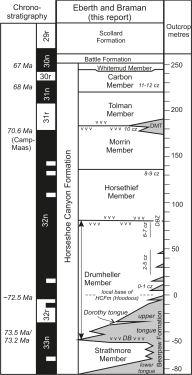
\includegraphics[width=\textwidth,height=0.4\textheight,keepaspectratio]{strat.png}
    \caption{A stratigraphic chart of the Horseshoe Canyon Formation. The RTMP is in the Drumheller member. Adapted from \cite[Fig.~2]{eberthRevisedStratigraphyDepositional2012}.}
    \label{fig:strat-chart}
\end{wrapfigure}

Below the HCF is the Bearpaw Formation, formed from marine sediments as the Western Interior Seaway rose to cover the land with water. Above it are the Battle and Scollard formations. The Scollard formation is particularly noteworthy as it contains the K-Pg extinction layer, a layer of sediment from 66 million years ago when an asteroid crashed into the area near Chixulub (Yucatan Peninsula), leading to the extinction of the non-avian dinosaurs \parencite{leckieScenicGeologyAlberta2021}.

The plant and animal life would have been abundant throughout the area. Imagine huge herds of hadrosaurs like \species{Edmontosaurus} and \species{Hypacrosaurus}, ceratopsians like \species{Anchiceratops} and ankylosaurs like \species{Euplocephalus} moving through the swamps and plains. They would have been observed by large predators like the tyrannosaurs \species{Albertosaurus}, while underfoot moved smaller species like the pachycephalosaur \species{Sphaeotholus} and the dromaeosaur \species{Atrociraptor} \parencite{eberthDinosaurBiostratigraphyEdmonton2013}.

The numerous dinosaurs, while the most charismatic animals in the area, certainly weren't the only ones! Turtles, while less common than in the warmer times immediately preceding and following, are still present \parencite{brinkmanReviewNonmarineTurtles2003}. In addition, mammals like the cat-sized \species{Didelphodon}, an early relative of marsupials, have been found \parencite{foxStagodontidMarsupialsLate2006}. Fish species, relative of modern-day gars and sturgeons among other, filled the streams and rivers \parencite{larsonFaunalAssemblagesUpper2010}.

While we often focus on the animal life of the HCF, the plant fossils that can be found in the area provide a fascinating glimpse into the environment at the time. It's very common when looking at the ironstone nodules found in the area to find fragments of sticks, needles, and pinecones from the numerous conifers that occurred at the time \parencite{serbetCunninghamiaTayloriiSp2013}. These ironstone nodules formed when particles began to accumulate around an object in the swamps, leading to beautiful preservation. These nodules frequently preserve their contents in three dimensions, allowing for exquisite fossils like an aroid flower to be preserved and studied \parencite{bognerFossilizedAroidInfructescence2005}. In addition, the fossil pollens in the area have been extensively studied, allowing us to understand the diversity and patterns of change throughout the seven million years of the HCF \parencite{kutlukMegasporesUpperCretaceous2017}. The plant fossils found around the RTMP paint a picture of an evolving landscape that transitioned from dry and cool to warm, wet, and tropical, then back to a more savannah-like environment.

\begin{figure}[H]
    \includegraphics[width=\textwidth]{horseshoeCanyonFormation.png}
    \caption{Artist's rendition of the area around Drumheller during the late Cretaceous. Image credit: Julius Csotonyi}
\end{figure}


One of the notable features of the HCF formation is that in certain areas, large bonebeds of species like \species{Edmontosaurus} or \species{Hypacrosaurus} are found \parencite{eberthRevisedStratigraphyDepositional2012, evansHadrosauridEdmontosaurusBonebeds2015}. The most famous of these is the \species{Albertosaurus} bonebed, located just north of the RTMP in Dry Island Buffalo Jump Provincial Park \parencite{eberthStratigraphySedimentologyTaphonomy2010}. This bonebed was discovered by famous fossil hunter Barnum Brown in 1910, lost, and then rediscovered in 1997 by a team from the RTMP and the Dinosaur International Society \parencite{curriePossibleEvidenceGregarious1998, spaldingDinosaursGraveyardCanadian1999}. It contains the remains of approximately 12 \species{Albertosaurus sarcophagus}, a smaller, faster relative of \species{Tyrannosaurus rex}, and may represent a family group. As terrifying as one \species{Albertosaurus} was, imagine a whole pack of them!

\begin{figure}[H]
\centering
\begin{subfigure}[b]{0.48\textwidth}
\centering
\includegraphics[width=\textwidth]{albertosaurus.jpeg}
    \caption{A model of an \species{Albertosaurus} family group at the RTMP}
\label{fig:albertosaurus}
\end{subfigure}
\hfill
\begin{subfigure}[b]{0.48\textwidth}
\centering
\includegraphics[width=\textwidth]{therrien-bonebed.jpeg}
    \caption{Dr. Fran\c{c}ois Therrien leading a tour of the \species{Albertosaurus} bonebed.}
\label{fig:therrien-bonebed}
\end{subfigure}
\end{figure}

However, in order for us to find all of these fossils, they needed to be exposed! The two main ways that new fossils are exposed around the RTMP are through the sudden erosion of the Red Deer River valley and the gradual erosion of the badlands. 

About \num{15000} years ago, much of Alberta (and the rest of Canada) was covered by glaciers more than \si{2}{km} thick \parencite[p.~170]{leckieScenicGeologyAlberta2021}. As these glaciers melted, the enormous volume of water carved deep river valleys, including the Red Deer river running through Drumheller. This exposed large portions of the fossil-rich HCF. Early fossils hunters in the area, such as Barnum Brown, routinely collected fossils by floating down the river and keeping an eye out for any exposed fossils along the riverbank or higher up in the valley \parencite[p.~47]{spaldingDinosaursGraveyardCanadian1999}. Even today it's not uncommon to find fossils while walking along the river!

\begin{figure}[H]
    \centering
    \includegraphics[width=0.5\textwidth]{amnh_scow.jpg}
    \caption{Barnum Brown and crew searching for fossils in the Red Deer river valley on a scow (1912).}
\end{figure}

In contrast to the (geologically) sudden carving out of the valley, the other process which exposes the fossils is erosion from wind and rain. In contrast to the humid, lush climate that would have been present 70 million years ago, the area around the RTMP today is dry and sparsely vegetated. The difficulty of making a living in this desolate climate led to the term 'badlands', but the misfortune of the early peoples in the area is a boon to palaeontologists! The lack of vegetation means that exposed fossils are easy to see, while simultaneously allowing the sparse rains in the area to erode away the solid and rock, exposing yet more fossils. The area can erode by as much as \si{4}{mm} a year \parencite{demers-potvinHighLocalVariability2025}, meaning that there is always a new crop of fossils to be found!

The area around the RTMP is one of the most extensively studied fossil sites on the planet. Thanks in large part to the museum's presence, it has become a hotbed of research on all aspects of this late-Cretaceous ecosystem, from the geology and climate on one hand to the plant and animal life on the other. Studies here have provided insights into the formation of the Rocky Mountains to the west and the Western Interior Seaway to the east. Having such extensive knowledge about this ancient ecosystem provides valuable insights into how changes in climate rippled through the interconnected web of species in the area. Even better, this treasure trove of information is publicly accessible, and in fact, a major tourist destination - a scientific legacy that we're fortunate to share in Alberta.

\section{References}
\begingroup
\renewcommand*{\bibfont}{\footnotesize}
\printbibliography[heading=none]
\endgroup

\end{document}
